\section{Lecture 5: Superscalar Architecture (SSA)}
Computer designed to improve computation on scalars instructions.
A scalar is a variable that can hold only one atomic value at a time, e.g., an integer or a real.
A scalar architecture processes one data item at a time -- the computers we discussed up till now.
Examples of non-scalar variables:
\begin{itemize}
\item Arrays -- Vector Processor
\item Matrices -- Graphics Processing Unit (GPU)
\item Records
\end{itemize}

In a superscalar architecture (SSA), several scalar instructions can be initiated simulaneously and executed independently.

\subsection{Instruction-level parallelism}
Most operations are on scalar quantities, speed up these operations will lead to large performance improvement.

\subsubsection{Superpipelining}
Superpipelining exploits the fact that many pipeline stages perform tasks that require less than half a clock cycle. Thus, a doubled internal clock speed allows the performance of two tasks in one external clock cycle.

We divide pipelining stages into several sub-stages, and hence increase the number of instructions which are handled by the pipeline at the same time. But note that although several instructions are executing concurrently, only one instruction is in its execution stage at any one time.

\todo{A picture would be nice here} \\

\begin{enumerate}
\item For example by diving each stage into two sub stages, we will be able (in the ideal situation) to perform each stage at twice the speed.
\item No duplication of hardware is needed. 
\item Not all stages can be divided into (equal length) sub stages.
\item Hazards more difficult to resolve.
\item More complex hardware.
\item Interrupt handling and testing will be more complicated.
\end{enumerate}
  
\subsubsection{Difference between Superpipelined and Superscalar Designs}
The difference is that Superpipeline can perform several instructions in one clock cycle, whereas Superscalar performs several instructions in parallel

\begin{figure}[H]
  \centering
  \scalebox{0.342}{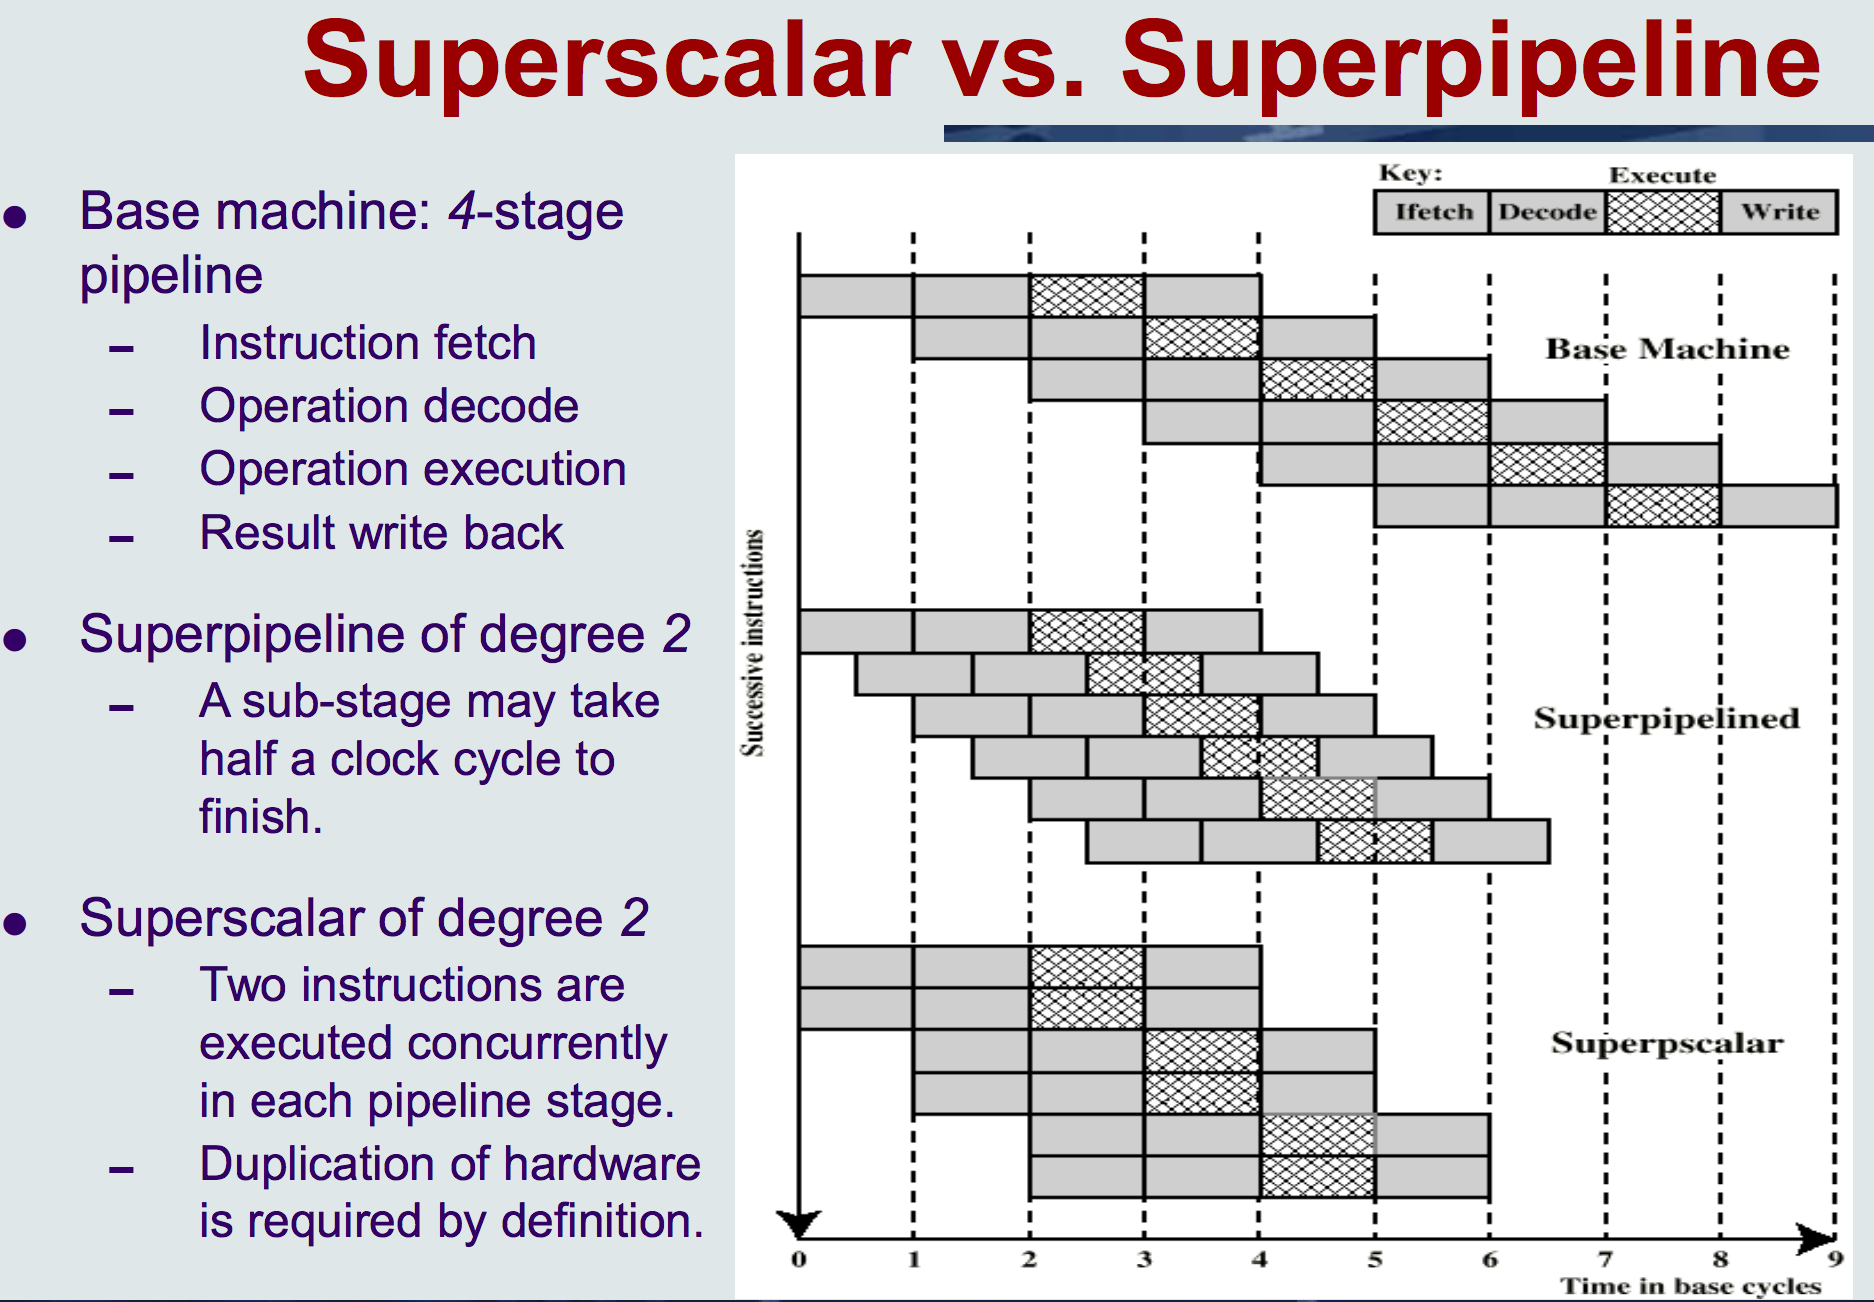
\includegraphics{img/superscalar-vs-superpipeline.png}}
  \caption{Difference between a Superscalar and a Superpipeline architecture}
  \label{fig:superscalar-vs-superpipeline}
\end{figure}


\subsubsection{Superscalar Superpipeline Design}

\begin{figure}[H]
  \centering
  \scalebox{0.342}{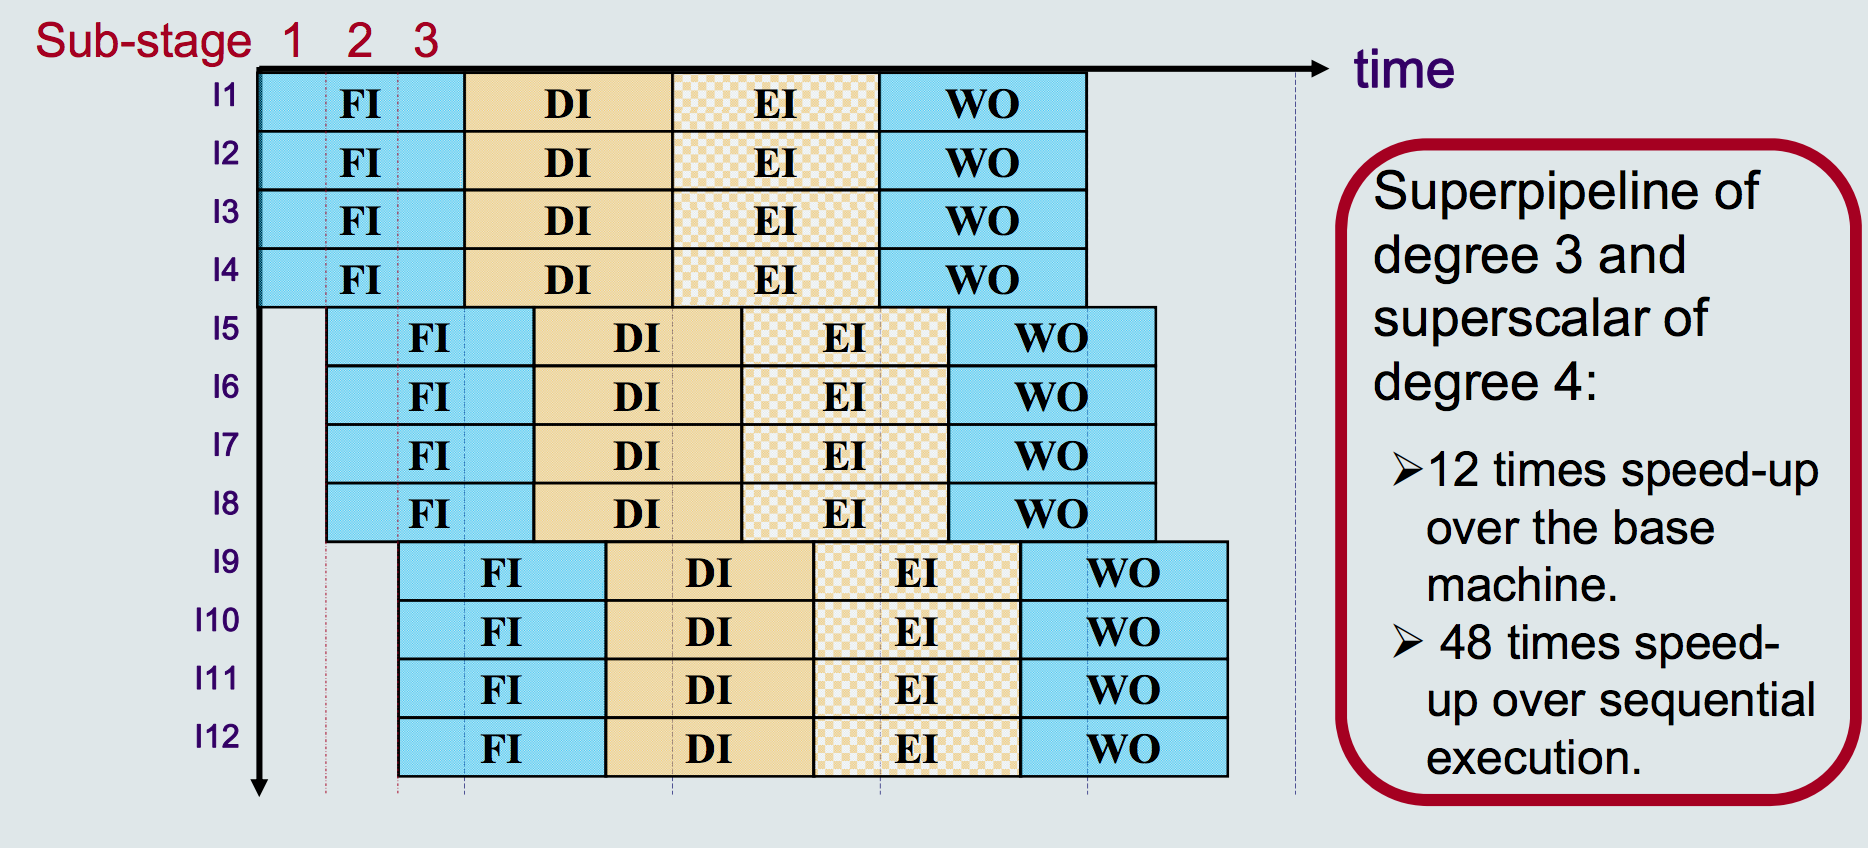
\includegraphics{img/superscalar-superpipeline.png}}
  \caption{Superscalar Superpipeline architecture}
  \label{fig:superscalar-superpipeline}
\end{figure}

The new trend is to combined the two ideas. In Figure \ref{fig:superscalar-superpipeline} it says that this would give us a 48 times speedup, this is not the case though because of data dependencies.

\subsection{Dependency issues}
The superscalar approach depends on the ability to execute multiple instructions in parallel. The term instruction-level parallelism refers to the degree to which, on average, the instructions of a program can be executed in parallel. A combination of compiler-based optimization and hardware techniques can be used to maximize instruction-level parallelism.

The main problems are:
\begin{itemize}
\item Resource conflicts.
\item Control (procedural) dependency.
\item Data dependencies.
\item True data dependency.
\item Output dependency.
\item Anti Dependency.
\end{itemize}
  
These are very similar to the cases in normal pipelining (data hazards). But the consequences are more severe here because the parallelism are greater and thus larger amount of performance will be lost.

\subsubsection{Resource Conflicts}
Several instructions compete for the same hardware resource at the same time.
\begin{itemize}
\item For instance, two aritmethic instructions need the same floating-point unit for execution.
\item similar to structural hazards in pipeline.
\end{itemize}

They can be solved \underline{partly} by introducing several hardware units for the same functions.
\begin{itemize}
\item e.g. have two floating point units.
\item the hardware units can also be pipelined to support several operations at the same time.
\item however, memory units \textbf{can't be duplicated}.
\end{itemize}
  
\subsubsection{Procedural Dependency}
\subsubsection{Data Conflicts}
\subsubsection{Window of execution}
\subsubsection{Data Dependencies}
All instructions in the window of execution may begin execution, subject to data dependence and resource constraints.
\begin{itemize}
\item True data dependency
\item Output dependency
\item Anti dependency
\end{itemize}

\subsubsection{True Data Dependency}
True data dependencies exist when the output of one instruction is required as an input to a subsequent instruction:
\begin{lstlisting}[frame=single]  % Start your code-block
  . . .
  MUL R4,R3,R1 (R4 := R3 * R1)
  . . .
  ADD R2,R4,R5 (R2 := R4 + R5)
\end{lstlisting}
In this example we can fetch and decode the second instruction in parallel, but we have to wait to perform it because its dependant on registers from the first instruction.

They are intrinsic features of a program, and cannot be eliminated by compiler or hardware techniques. The hardware have to detect them, and solve them. The easiest way to do this in this example, is just to stall the first instruction until we can perform the second.

This type of depency is very common, and by increasing the window size we can reduce the impact of them.
\subsubsection{Output Dependency}
\subsubsection{Anti Dependency}
\subsubsection{Effect of Dependencies}
\subsection{Parallel instruction execution}
\subsubsection{Instruction vs Machine Parallelism}
\subsubsection{Division and Decoupling}
\subsubsection{SSA instruction Execution Policies}
\subsubsection{In-Order with In-Order Completion}
This seems important to understand
\subsubsection{In-Order issue with Out-of-Order Completion}
This seems important to understand
